\documentclass[fleqn]{article}
\usepackage[nodisplayskipstretch]{setspace}
\usepackage{amsmath, nccmath, bm}
\usepackage{amssymb}
\usepackage{enumitem}
\usepackage{graphicx}
\usepackage{float}
\usepackage{caption}

\newcommand{\zerodisplayskip}{
	\setlength{\abovedisplayskip}{0pt}%
	\setlength{\belowdisplayskip}{0pt}%
	\setlength{\abovedisplayshortskip}{0pt}%
	\setlength{\belowdisplayshortskip}{0pt}%
	\setlength{\mathindent}{0pt}}
	
\newcommand{\norm}[1]{\left \lVert #1 \right \rVert}

\makeatletter
	\newenvironment{equationCenter}{\@fleqnfalse\begin{equation*}}{\end{equation*}}
\makeatother

\title{Final Exam}
\author{Owen Sowatzke}
\date{December 12, 2024}

\begin{document}

	\offinterlineskip
	\setlength{\lineskip}{12pt}
	\setcounter{MaxMatrixCols}{20}
	\zerodisplayskip
	\maketitle
	
	\begin{enumerate}
		\item In Figure 1 is shown a $2 \times 2$ polarization-time coding MIMO scheme, which employs dual-polarization transmit and receive antennas. Due to multipath effect, the initial orthogonality of polarization states is no longer preserved on a receiver side and we can use the channel coefficients as shown in Fig. 1 to describe this depolarization effect. Show that Alamouti $2 \times 2$ scheme can be used to deal with depolarization effect. Determine the array, diversity and multiplexing gains of this scheme. How would you determine the channel capacity of this scheme? Consider now a MIMO scheme employing two dual-polarization Tx antennas and two dual-polarization Rx antennas. How would approach this system to deal simultaneously with depolarization and multipath effects? How would you determine the channel capacity of this scheme?

		\begin{figure}[H]
			\centerline{\fbox{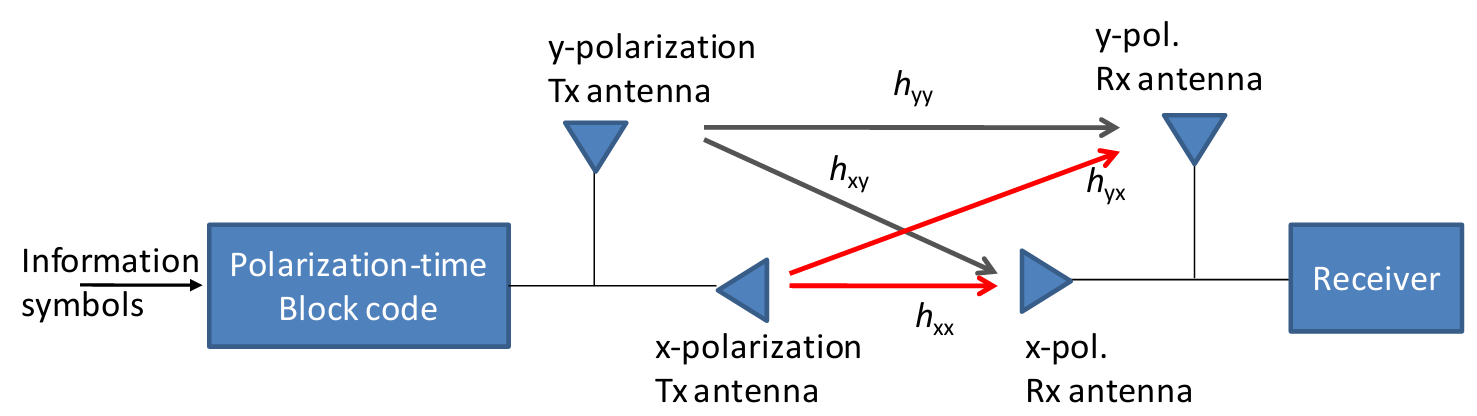
\includegraphics[width=0.8\textwidth]{2x2_polarization_time_coding_mimo.png}}}
			\caption{}
			\label{fig::2x2_polarization_time_coding_mimo}
		\end{figure}
		
%		In a MIMO system, the Alamouti $2\times 2$ scheme is implemented using the following code matrix:
%		
%		\begin{equation*}
%			\mathbf{X} = \begin{bmatrix}
%				x_1 & -x_2^*\\
%				x_2 & x_1^*
%			\end{bmatrix}
%		\end{equation*}
%		
%		In the first channel use, the antenna $T_{x_1}$ transmits $x_1$, and the antenna $T_{x_2}$ transmits $x_2$. In the second channel use, the antenna $T_{x_1}$ transmits $-x_2^*$ and the antenna $T_{x_2}$ transmits $x_1^*$.
%		
%		For a dual polarization system, we can leverage the Alamouti in a similar manner to determine to deal with the depolarization effect. In the first channel use, we send $s_x$ on the the x-polarization antenna and $s_y$ on the y-polarization antenna. In the second channel use, we send $-s_y^*$ on the x-polarization antenna and $s_x^*$ on the y-polarization antenna.
%		
%		The received signal vectors for the first and second channel use are denoted as $\mathbf{r_{i,1}}$ and $\mathbf{r_{i,2}}$ and are denoted as follows:
%		
%		\begin{equation*}
%			\mathbf{r_{i,1}} = \mathbf{Hs_{i,1}}e^{j(\phi_T - \phi_{LO}) + j\phi_{CD}(k)}
%		\end{equation*}
%		
%		\begin{equation*}
%			\mathbf{r_{i,2}} = \mathbf{Hs_{i,2}}e^{j(\phi_T - \phi_{LO}) + j\phi_{CD}(k)}
%		\end{equation*}\\
%		
%		 The transmitted symbols are now denoted as $s_x$ and $s_y$, and we use $\mathbf{S}$ to denote the code matrix.
%		
%		\begin{equation*}
%			\mathbf{S} = \begin{bmatrix}
%				s_x & -s_y^*\\
%				s_y & s_x^*
%			\end{bmatrix}
%		\end{equation*}
%		
%		FUCK
%		
%		\pagebreak
		
		\begin{equation*}
			\begin{bmatrix}
				r_{x,1} & r_{x,2} \\
				r_{y,1} & r_{y,2}
			\end{bmatrix} = \begin{bmatrix}
				h_{xx} & h_{xy} \\
				h_{yx} & h_{yy}
			\end{bmatrix}\begin{bmatrix}
				s_x & -s_y^* \\
				s_y & s_x^*
			\end{bmatrix} + \begin{bmatrix}
				n_{x,1} & n_{x,2} \\
				n_{y,1} & n_{y,2}
			\end{bmatrix}
		\end{equation*}
			
		\begin{equation*}
				 = \begin{bmatrix}
				h_{xx}s_x + h_{xy}s_y & -h_{xx}s_y^* + h_{xy}s_x^* \\
				h_{yx}s_x + h_{yy}s_y & -h_{yx}s_y^* + h_{yy}s_x^*
			\end{bmatrix} + \begin{bmatrix}
				n_{x,1} & n_{x,2} \\
				n_{y,1} & n_{y,2}
			\end{bmatrix}
		\end{equation*}
		
		We can estimate the transmitted symbols as follows:
		
		\begin{equation*}
			\tilde{s}_x = h_{xx}^*r_{x,1} + h_{xy}r_{x,2}^* + h_{yx}^*r_{y,1} + h_{yy}r_{y,2}^*
		\end{equation*}
		
		\begin{equation*}
			\tilde{s}_y = h_{xy}^*r_{x,1} - h_{xx}r_{x,2}^* + h_{yy}^*r_{y,1} - h_{yx}r_{y,2}^*
		\end{equation*}
		
		Substituting, we obtain:
		
		\begin{equation*}
			\tilde{s}_x = h_{xx}^*(h_{xx}s_x + h_{xy}s_y) + h_{xy}(-h_{xx}^*s_y + h_{xy}^*s_x) + h_{yx}^*(h_{yx}s_x + h_{yy}s_y)
		\end{equation*}
		
		\begin{equation*}
			 + h_{yy}(-h_{yx}^*s_y + h_{yy}^*s_x) + \text{noise}
		\end{equation*}
		
		\begin{equation*}
			= |h_{xx}|^2s_x + h_{xx}^*h_{xy}s_y - h_{xx}^*h_{xy}s_y + |h_{xy}|^2s_x + |h_{yx}|^*s_x + h_{yx}^*h_{yy}s_y
		\end{equation*}
		
		\begin{equation*}
			- h_{yx}^*h_{yy}s_y + |h_{yy}|^2s_x + \text{noise}
		\end{equation*}
		
		\begin{equation*}
			= (|h_{xx}|^2 + |h_{xy}|^2 + |h_{yx}|^2 + |h_{xy}|^2)s_x + \text{noise}
		\end{equation*}
		
		\begin{equation*}
			\tilde{s}_y = h_{xy}^*r_{x,1} - h_{xx}r_{x,2}^* + h_{yy}^*r_{y,1} - h_{yx}r_{y,2}^*
		\end{equation*}
		
		\begin{equation*}
			= h_{xy}^*(h_{xx}s_x + h_{xy}s_y) - h_{xx}(-h_{xx}^*s_y + h_{xy}^*s_x) + h_{yy}^*(h_{yx}s_x + h_{yy}s_y)
		\end{equation*}
		
		\begin{equation*}
			- h_{yx}(-h_{yx}^*s_y + h_{yy}^*s_x) + \text{noise}
		\end{equation*}
		
		\begin{equation*}
			= h_{xx}h_{xy}^*s_x + |h_{xy}|^2s_y + |h_{xx}|^2s_y - h_{xx}h_{xy}^*s_x + h_{yx}h_{yy}^*s_x + |h_{yy}|^2s_y
		\end{equation*}
		
		\begin{equation*}
			+ |h_{yx}|^2s_y - h_{yx}h_{yy}^*s_x + \text{noise}
		\end{equation*}
		
		\begin{equation*}
			= (|h_{xx}|^2 + |h_{xy}|^2 + |h_{yx}|^2 + |h_{yy}|^2)s_y + \text{noise}
		\end{equation*}
		
		Looking at $\tilde{s}_x$ and $\tilde{s}_y$, we can see that the Alamouti $2\times 2$ scheme effectively deals with the depolarization effect.
		
		\pagebreak
		
%		The spatial interference is accounted for but the noise power is increased by a factor of 4. The received SNR is given by:
%		
%		\begin{equation*}
%			\rho = \frac{(|h_{xx}|^2 + |h_{xy}|^2 + |h_{yx}|^2 + |h_{yy}|^2)}{4}\frac{E_s}{N_0}
%		\end{equation*}
%		
%		The received SNR is 1/4 the sum of SNR's from 
%		The array gain is 1, 

		Array gain of Almouti scheme is $M_{RX}$ and diversity gain is $M_{TX}M_{RX}$.
		
		Thus, for a $2 \times 2$ Almouti scheme, the array gain is 2 and the diversity gain is 4.
		
		The Almouti scheme also prioritizes diversity over multiplexing gain. As such, the multiplexing gain for this system is 1.	
		
		In an Almouti scheme, we only have CSIR. We also consider the effects of fading, since there is a multi-path effect. Therefore, we consider the ergodic channel capacity.
		
		\begin{equation*}
			C = \underset{\mathbf{R_x}:\ Tr(\mathbf{R_x}) = \rho}{\text{max}}\left\langle W \text{log}_2[\text{det}(\mathbf{I} + \mathbf{HR_xH^{\dagger}})]\right\rangle_{\mathbf{H}}
		\end{equation*}
		
		The optimum input covariance that maximizes ergodic channel capacity is the scaled identity matrix, so that ergodic channel capacity can be written as:
		
		\begin{equation*}
			C = \left\langle W \text{log}_2\left[\text{det}\left(\mathbf{I} + \frac{\bar{\rho}}{M_{Tx}}\mathbf{HH^{\dagger}}\right)\right]\right\rangle_{\mathbf{H}}
		\end{equation*}
		
%		\begin{equation*}
%			
%		\end{equation*}
		
		To handle simultaneously deal with depolarization and multipath effects, we can employ a $4 \times 4$ MIMO techniques. Specifically, we can use $4 \times 4$ space-time code to simultaneously deal with depolarization and multipath effects.
		
		For space-time block coding, we have
		
		\begin{equation*}
			\mathbf{Y} = \mathbf{HX}
		\end{equation*}
			
		where $Y$ is the received vector and $\mathbf{X}$ is the transmit 
		
		\item An $(n,k)$ linear block code is described by the following parity-check matrix:
		
		\begin{equationCenter}
			\mathbf{H} = \begin{bmatrix}
				0 & 0 & 0 & 0 & 0 & 0 & 0 & 1 & 1 & 1 & 1 & 1 & 1 & 1 & 1 \\
				0 & 0 & 0 & 1 & 1 & 1 & 1 & 0 & 0 & 0 & 0 & 1 & 1 & 1 & 1 \\
				0 & 1 & 1 & 0 & 0 & 1 & 1 & 0 & 0 & 1 & 1 & 0 & 0 & 1 & 1 \\
				1 & 0 & 1 & 0 & 1 & 0 & 1 & 0 & 1 & 0 & 1 & 0 & 1 & 0 & 1
			\end{bmatrix}
		\end{equationCenter}
		
		\begin{enumerate}
			\item Determine the code parameters of this code: codeword length, number of information bits, code rate, overhead, minimum distance, error correction capability, and error detection capability.
			
			$\mathbf{H}$ is a $(n-k) \times n$ matrix.

			$\Rightarrow n = 15,\ k = 11$
						
			Codeword length: $n = 15\ \text{bits}$
			
			Number of information bits: $k = 11\ \text{bits}$
			
			Code rate: $R = k/n = 11/15$
			
			Overhead: $n - k = 4\ \text{bits}$
			
			The minimum distance of a linear block code is defined by the minimum number of columns of the $\mathbf{H}$-matrix whose sum is equal to the zero vector:
			
			The first 3 columns of the provided $\mathbf{H}$-matrix sum to the zero vector, and there are no duplicated columns.
			
			$\therefore$ Minimum distance: $d_\text{min} = 3$
			
			Error correction capability and error detection capability are related to the minimum distance by
			
			\begin{equation*}
				d_{\text{min}} = \geq e_d + e_c + 1
			\end{equation*}
			
			where $e_d$ is the number of detected errors and $e_c$ is the number of corrected errors.
			
			To determine error correction capability, we must set $e_d = e_c$ because we must detect the errors in all the bits we correct.
			
			\begin{equation*}
				\Rightarrow d_{\text{min}} \geq 2e_c + 1 \Rightarrow 2e_c \leq d_{\text{min}} - 1 \Rightarrow e_c \leq 1
			\end{equation*}
			
			$\therefore$ we can correct up to 1 bits in error.
			
			To determine error detection capability, we must set $e_c = 0$ because we are only responsible for detecting errors.
			
			\begin{equation*}
				\Rightarrow d_{\text{min}} \geq e_d + 1 \Rightarrow e_d \leq d_{\text{min}} - 1 \Rightarrow e_d \leq 2
			\end{equation*}
			
			$\therefore$ we can detect up to 2 bits in error.
			
			Note that for this code, we cannot simultaneously correct 1 bit and detect 2 errors. We can either do single bit error correction \textbf{\underline{or}} 2 bit error detection.
			
			%\begin{equation*}

			\pagebreak
			\item Represent the $\mathbf{H}$-matrix in systematic form and determine the generator matrix $\mathbf{G}$ of the corresponding systematic code. Provide the corresponding shift register based encoding circuit of this systematic code.
			
			The systematic form of $\mathbf{H}$ is given as follows:
			
			\begin{equation*}
				\mathbf{H} = \left[\begin{array}{c|c}
					\mathbf{P^T} & \mathbf{I}
				\end{array}\right]
			\end{equation*}
			
			We should be able to use row operations and column permutations to put $\mathbf{H}$ in the requested form. The columns of $\mathbf{H}$ that form an identity matrix are already present. Using column permutations, we can find the systematic form, which is given below:
			
			\begin{equation*}
				\mathbf{H} = \begin{bmatrix}
					0 & 0 & 0 & 0 & 1 & 1 & 1 & 1 & 1 & 1 & 1 & 1 & 0 & 0 & 0 \\
					0 & 1 & 1 & 1 & 0 & 0 & 0 & 1 & 1 & 1 & 1 & 0 & 1 & 0 & 0 \\
					1 & 0 & 1 & 1 & 0 & 1 & 1 & 0 & 0 & 1 & 1 & 0 & 0 & 1 & 0 \\
					1 & 1 & 0 & 1 & 1 & 0 & 1 & 0 & 1 & 0 & 1 & 0 & 0 & 0 & 1
				\end{bmatrix}
			\end{equation*}
		
			The systematic generator matrix $\mathbf{G}$ is now given as follows:
			
			\begin{equation*}
				\mathbf{G} = \left[\begin{array}{c|c}
					\mathbf{I} & \mathbf{P}
				\end{array}\right]
			\end{equation*}
			
			\begin{equation*}
				\mathbf{G} = \begin{bmatrix}
					1 & 0 & 0 & 0 & 0 & 0 & 0 & 0 & 0 & 0 & 0 & 0 & 0 & 1 & 1\\
					0 & 1 & 0 & 0 & 0 & 0 & 0 & 0 & 0 & 0 & 0 & 0 & 1 & 0 & 1\\
					0 & 0 & 1 & 0 & 0 & 0 & 0 & 0 & 0 & 0 & 0 & 0 & 1 & 1 & 0\\
					0 & 0 & 0 & 1 & 0 & 0 & 0 & 0 & 0 & 0 & 0 & 0 & 1 & 1 & 1\\
					0 & 0 & 0 & 0 & 1 & 0 & 0 & 0 & 0 & 0 & 0 & 1 & 0 & 0 & 1\\
					0 & 0 & 0 & 0 & 0 & 1 & 0 & 0 & 0 & 0 & 0 & 1 & 0 & 1 & 0\\
					0 & 0 & 0 & 0 & 0 & 0 & 1 & 0 & 0 & 0 & 0 & 1 & 0 & 1 & 1\\
					0 & 0 & 0 & 0 & 0 & 0 & 0 & 1 & 0 & 0 & 0 & 1 & 1 & 0 & 0\\
					0 & 0 & 0 & 0 & 0 & 0 & 0 & 0 & 1 & 0 & 0 & 1 & 1 & 0 & 1\\
					0 & 0 & 0 & 0 & 0 & 0 & 0 & 0 & 0 & 1 & 0 & 1 & 1 & 1 & 0\\
					0 & 0 & 0 & 0 & 0 & 0 & 0 & 0 & 0 & 0 & 1 & 1 & 1 & 1 & 1
				\end{bmatrix}
			\end{equation*}
			
			The codeword is given as follows:
			
			\begin{equation*}
				\mathbf{x} = \begin{bmatrix}{\begin{array}{c|c}
					\mathbf{m} & \mathbf{b}			
				\end{array}}\end{bmatrix} = \mathbf{m}\begin{bmatrix}
					\begin{array}{c|c}
						\mathbf{I} & \mathbf{P}
					\end{array}
				\end{bmatrix} = \mathbf{mG} 
				\Rightarrow \mathbf{b} = \mathbf{mP}
			\end{equation*}
			
			The parity bits are given as follows:
			
			\begin{equation*}
				b_0 = p_{4,0}m_{4} + p_{5,0}m_{5} + p_{6,0}m_{6} + p_{7,0}m_{7} + p_{8,0}m_{8} + p_{9,0}m_{9} + p_{10,0}m_{10}
			\end{equation*}
			
			\begin{equation*}
				b_1 = p_{1,1}m_{1} + p_{2,1}m_{2} + p_{3,1}m_{3} + p_{7,0}m_{7} + p_{8,1}m_{8} + p_{9,1}m_{9} + p_{10,1}m_{10}
			\end{equation*}
			
			\begin{equation*}
				b_2 = p_{0,2}m_{0} + p_{2,2}m_{2} + p_{3,2}m_{3} + p_{5,3}m_{5} + p_{6,3}m_{6} + p_{9,3}m_{9} + p_{10,3}m_{10}
			\end{equation*}
			
			\begin{equation*}
				b_3 = p_{0,3}m_{0} + p_{1,3}m_{1} + p_{3,3}m_{3} + p_{4,3}m_{4} + p_{6,3}m_{6} + p_{8,3}m_{8} + p_{10,3}m_{10}
			\end{equation*}
			
			\item The extended code is created by inserting the additional parity-check bits. The most common way of extending the code is by adding an overall parity-check bit. The extended code is then an $(n+1,k)$ code. Determine the bipartite (Tanner) graph of $\mathbf{H}$-matrix of extended code obtained from the original $\mathbf{H}$-matrix above.
			
			We can XOR the bits of the parity matrix to add an even overall parity check-bit.
			
			\begin{equation*}
				\mathbf{P} = \begin{bmatrix}
					0 & 0 & 1 & 1 & 1 \\
					0 & 1 & 0 & 1 & 1 \\
					0 & 1 & 1 & 0 & 1 \\
					0 & 1 & 1 & 1 & 0 \\
					1 & 0 & 0 & 1 & 1 \\
					1 & 0 & 1 & 0 & 1 \\
					1 & 0 & 1 & 1 & 0 \\
					1 & 1 & 0 & 0 & 1 \\
					1 & 1 & 0 & 1 & 0 \\
					1 & 1 & 1 & 0 & 0 \\
					1 & 1 & 1 & 1 & 1
				\end{bmatrix}
			\end{equation*}
			
			The parity-check matrix is now given as follows:
			
			\begin{equation*}
				\mathbf{H} = \begin{bmatrix}
					0 & 0 & 0 & 0 & 1 & 1 & 1 & 1 & 1 & 1 & 1 & 1 & 0 & 0 & 0 & 0\\
					0 & 1 & 1 & 1 & 0 & 0 & 0 & 1 & 1 & 1 & 1 & 0 & 1 & 0 & 0 & 0\\
					1 & 0 & 1 & 1 & 0 & 1 & 1 & 0 & 0 & 1 & 1 & 0 & 0 & 1 & 0 & 0\\
					1 & 1 & 0 & 1 & 1 & 0 & 1 & 0 & 1 & 0 & 1 & 0 & 0 & 0 & 1 & 0\\
					1 & 1 & 1 & 0 & 1 & 1 & 0 & 1 & 0 & 0 & 1 & 0 & 0 & 0 & 0 & 1
				\end{bmatrix}
			\end{equation*}
				
			\begin{figure}[H]
				\centerline{\fbox{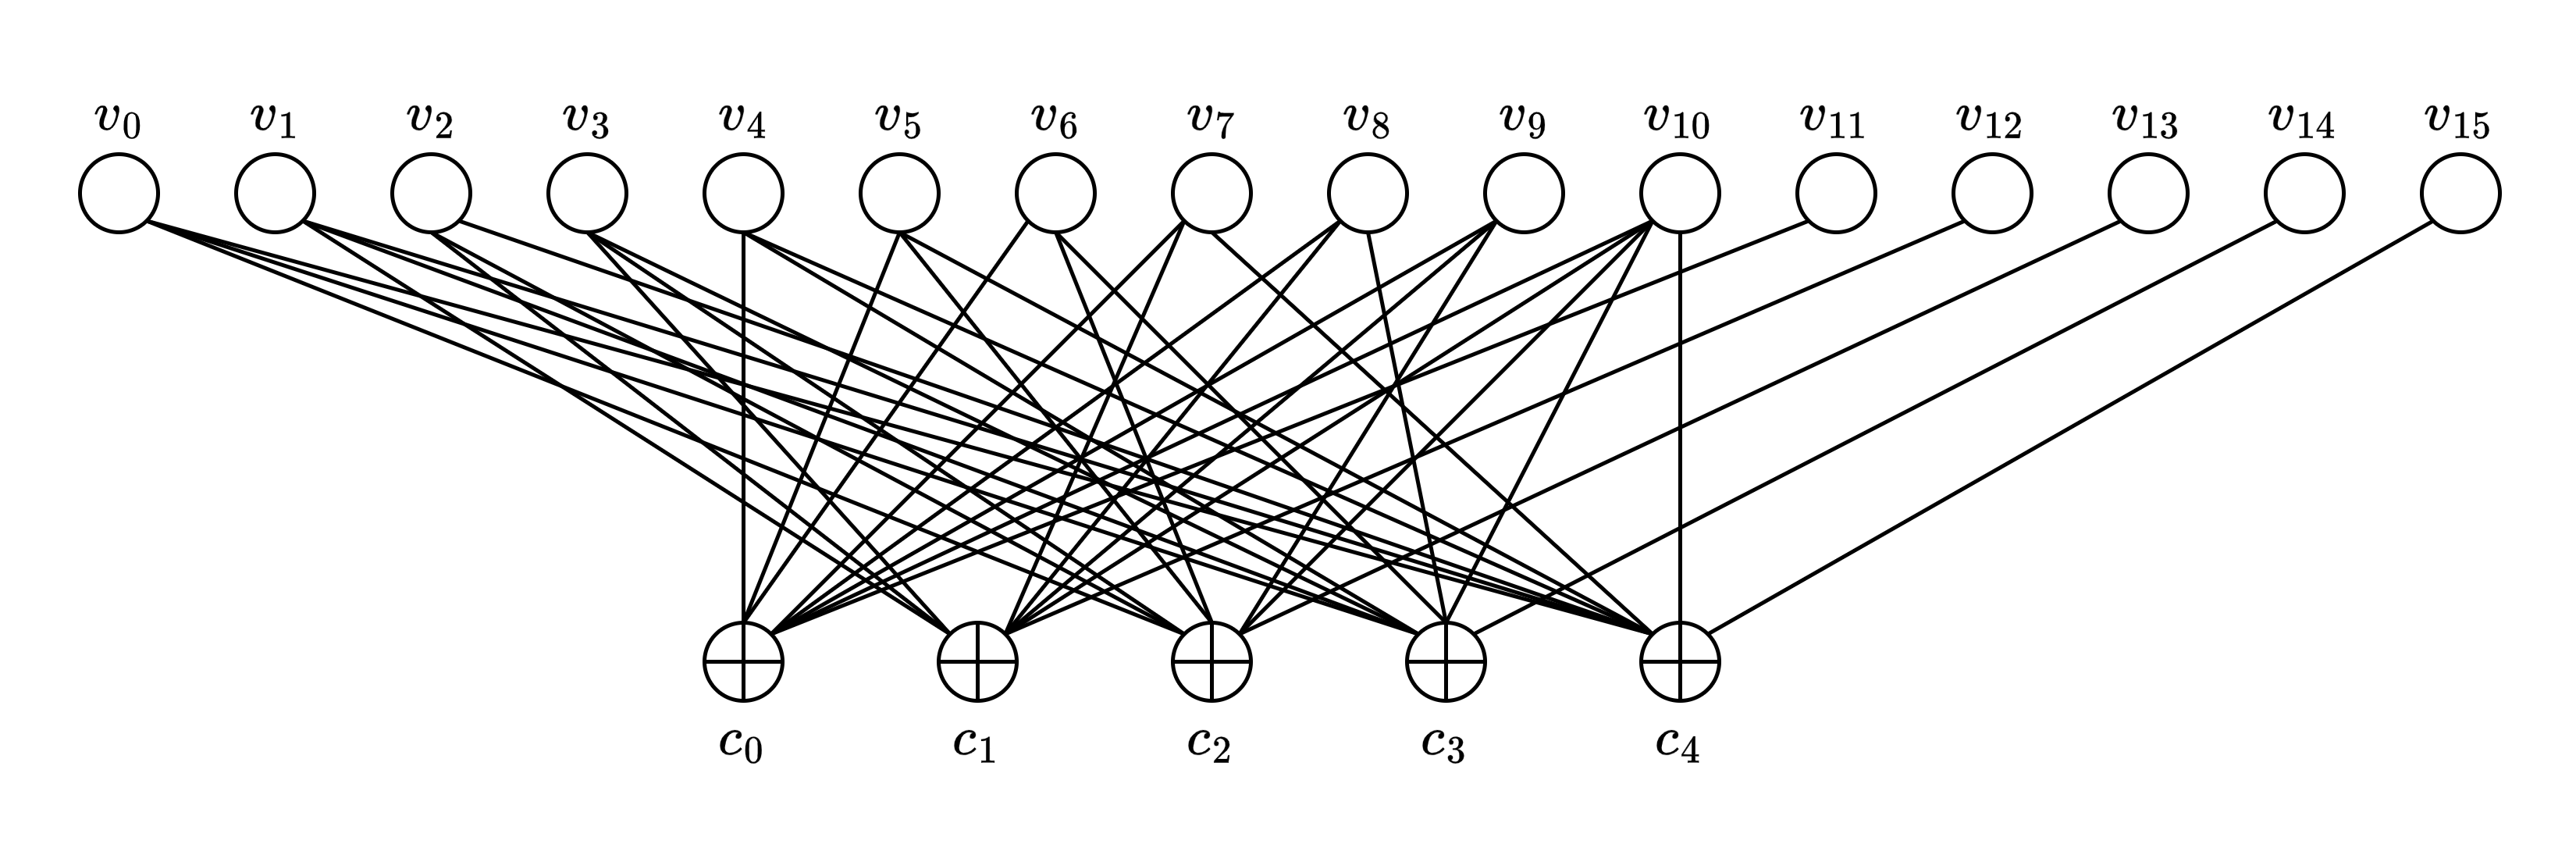
\includegraphics[width=0.8\textwidth]{tanner_graph.png}}}
				\caption{Tanner Graph}
				\label{fig::tanner_graph}
			\end{figure}

			\item Determine the code parameters of the extended code in (c): codeword length, number of information bits, code rate, overhead, minimum distance, error correction capability, and error detection capability.
			
			$\Rightarrow n = 15,\ k = 11$
						
			Codeword length: $n + 1 = 16\ \text{bits}$
			
			Number of information bits: $k = 11\ \text{bits}$
			
			Code rate: $R = k/(n+1) = 11/16$
			
			Overhead: $n - k = 5\ \text{bits}$
			
			The minimum distance of a linear block code is defined by the minimum number of columns of the $\mathbf{H}$-matrix whose sum is equal to the zero vector:
			
			Minimum distance: $d_\text{min} = 4$
			
			Error correction capability and error detection capability are related to the minimum distance by
			
			\begin{equation*}
				d_{\text{min}} = \geq e_d + e_c + 1
			\end{equation*}
			
			where $e_d$ is the number of detected errors and $e_c$ is the number of corrected errors.
			
			To determine error correction capability, we must set $e_d = e_c$ because we must detect the errors in all the bits we correct.
			
			\begin{equation*}
				\Rightarrow d_{\text{min}} \geq 2e_c + 1 \Rightarrow 2e_c \leq d_{\text{min}} - 1 \Rightarrow e_c \leq 1.5
			\end{equation*}
			
			$\therefore$ we can correct up to 1 bits in error.
			
			To determine error detection capability, we must set $e_c = 0$ because we are only responsible for detecting errors.
			
			\begin{equation*}
				\Rightarrow d_{\text{min}} \geq e_d + 1 \Rightarrow e_d \leq d_{\text{min}} - 1 \Rightarrow e_d \leq 3
			\end{equation*}
			
			$\therefore$ we can detect up to 3 bits in error.
			
			Note that for this code, we cannot simultaneously correct 1 bit and detect 3 errors. However, we can do single bit error correction and detect a single uncorrected bit \textbf{\underline{or}} we can do 3 bit error detection.
		\end{enumerate}
		
		\item This problem is related to the \textbf{adaptive modulation and coding applied to 9-ary 2-D constellation} described below, transmitted over wireless channel in the presence of Nakagami fading and AWGN. The eight constellation points in this 2-D constellation are placed on a circle of radius 1. The last (ninth) point is placed in the origin. Assume that the point in the origin appears with probability 0.5, all others with probability 0.5/8. For channel coding use the extended code from Problem 2(c).
		
		\begin{enumerate}
			\item Determine the average symbol error probability for this modulation format in the presence of fading and AWGN.
			
			The average symbol energy is defined by:
			
			\begin{equation*}
				E_{av} = \sum_{i=1}^{9}{p_iE_i} = \sum_{i=1}^{9}{p_i\norm{\mathbf{s_i}}^2} = 0.5(0) + 8(0.5/8)(1) = 0.5
			\end{equation*}
			
			The symbol error probability in an AWGN channel can be expressed as follows:
			
			\begin{equation*}
				P_e = \sum_{i=1}^{9}{p_iP_e(m_i)}
			\end{equation*}
				
			For sufficiently high SNR, we can estimate $P_e(m_i)$ with the nearest neighbor approximation.
			
			\begin{equation*}
				P_e(m_i) \approx M_{dmin}Q\left(\frac{d_{min}}{\sqrt{2N_0}}\right)
			\end{equation*}
			
			where $M_{dmin}$ is the number of nearest nearest neighbors to the constellation point of interest and $d_{min}$ is the distance to the nearest neighbors.
			
			For the constellation point at the origin:
			
			\begin{equation*}
				P_e(m_1) \approx 8Q\left(\frac{\sqrt{2E_{av}}}{{\sqrt{2N_0}}}\right) = 8Q(\sqrt{\rho})
			\end{equation*}
			
			For the constellation points on the circle:
			
			\begin{equation*}
				P_e(m_i) \approx 2Q\left(\frac{\sqrt{2E_{av}}(2\text{sin}(\pi/8))}{{\sqrt{2N_0}}}\right) = 2Q(2\sqrt{\rho}\text{sin}(\pi/8))\ \forall\ 2 \leq i \leq 9
			\end{equation*}
			
			where $\rho$ is the SNR of the symbol.
			
			$\therefore$, assuming high SNR, we can estimate the symbol error in an AWGN channel as follows:
			
			\begin{equation*}
				P_s(\rho) \approx (0.5)8Q(\sqrt(\rho)) + (0.5/8)(8)2Q(2\sqrt{\rho}\text{sin}(\pi/8))
			\end{equation*}
			
			\begin{equation*}
				= 4Q(\sqrt{\rho}) + Q(2\sqrt{\rho}\text{sin}(\pi/8))
			\end{equation*}
			
			We can integrate the probability of symbol error over the fading distribution to get the average symbol error probability.
			
			\begin{equation*}
				\bar{P}_s = \int_{0}^{\infty}{P_s(\rho)f_{\rho}(\rho)d\rho}
			\end{equation*}
			
			\begin{equation*}
				\approx \int_{0}^{\infty}{(4Q(\sqrt{\rho}) + Q(2\sqrt{\rho}\text{sin}(\pi/8)))\left(\frac{m}{\bar{\rho}}\right)^m\frac{\rho^{m-1}}{\Gamma(m)}\text{exp}\left(-\frac{m\rho}{\bar{\rho}}\right)d\rho}
			\end{equation*}
			
			where $m$ is the fading figure.
			
			\item Estimate the coding gain for the extended code from Problem 2(c) and use it in incoming (c)-(e) problems.
			
			The coding gain when a \textbf{\underline{hard decision}} is applied in the coding process is given as follows:
			
			\begin{equation*}
				G_h[\text{dB}] = 10\text{log}_{10}[r(t+1)] = 10\text{log}_10\left[\frac{11}{16}(1+1)\right] = 1.3830 \ \text{dB}
			\end{equation*}
				
			The coding gain when a \textbf{\underline{soft decision}} is applied in the coding process is given as follows:
			
			\begin{equation*}
				G_s[\text{dB}] = 10\text{log}_{10}[rd_{min}] = 10\text{log}_10\left[\frac{11}{16}(4)\right] = 4.3933 \ \text{dB}
			\end{equation*}
			
			\item Determine the optimum power adaptation strategy as well as the corresponding the spectral efficiency of this scheme, in the presence of fading and AWGN.
			
			% Not sure if this is right.
			
%			The optimum power adaptation policy is given by
%			
%			\begin{equation*}
%				\frac{P(\rho)}{\bar{P}} = \begin{cases}
%					1/\rho_{tsh} - 1/\rho K, & \rho \geq p_{tsh}/K \\
%					0, & \rho < \rho_{tsh}/K
%				\end{cases}
%			\end{equation*}
%			
%			where 
			\item Describe the channel inversion technique for this signal constellation and determine the corresponding spectral efficiency, in the presence of fading and AWGN.
			
			\item Describe the truncated channel inversion technique for this signal constellation and determine the corresponding spectral efficiency, in the presence of fading and AWGN.
		\end{enumerate}
		
		\item In this problem we are concerned with designing an OFDM system that can provide data rate $\geq 50$ Mb/s for available bandwidth of 20 MHz, and which can tolerate the delay spread of up to 100 ns. Provide the design of such a system and describe the corresponding OFDM transceiver.
		
		The guard time should be 2-4 times RMS of delay spread.
		
		Let guard time be $4\times$ RMS of delay spread.
		
		\begin{equation*}
			\Rightarrow \text{Guard Time} = \mathbf{400\ ns}
		\end{equation*}
		
		Symbol duration should be at least $5\times$ the guard time. 
		
		Let symbol duration be $5\times$ guard time
		
		\begin{equation*}
			\Rightarrow \text{Symbol Duration} = \mathbf{2.0\ \mu{s}}
		\end{equation*}
		
		Subcarrier spacing:
		
		\begin{equation*}
			{\Delta}f_{sc} = 1/(T_s - T_G) = \mathbf{625\ \text{\textbf{kHz}}}
		\end{equation*}
		
		Number of carriers = (the required bit rate) / (OFDM symbol rate)
		
		= (the required bit rate) * (OFDM symbol duration)
		 
		\begin{equation*}
			= 50\ \text{Mbps} \times 2.0\ {\mu}s = \mathbf{100\ \text{\textbf{bits per OFDM symbol}}}
		\end{equation*}
		
		Determine the \underline{maximum} number of subcarriers.
		
		\begin{equation*}
			\frac{20\ \text{MHz}}{625\ \text{kHz}} = 32\ \text{subcarriers}
		\end{equation*}
		
		Consider 64-QAM with 5/6 rate coding (5 bits per symbol per subcarrier).
		
		\begin{equation*}
			\Rightarrow \mathbf{20}\ \text{\textbf{subcarriers}}
		\end{equation*}
		
		The bandwidth occupied with be
		
		$20 \times 625\ \text{kHz} = 12.5\ \text{MHz} < 20\ \text{MHz}$
		
		Additional advantage: 32-point radix-2 FFT/IFFT can be used, leaving 12 zero subcarriers to provide oversampling.
		
		An additional requirement is that an integer number of samples must be used within FFT/IFFT interval and in the symbol interval.
		
		Let the number of samples per symbol be $40$ samples.
		
		\begin{equation*}
			\Rightarrow \text{Sampling Rate} = 40/2.0{\mu}s = \mathbf{20}\ \text{\textbf{MHz}}
		\end{equation*}
		
		Then, the FFT/IFFT interval will be
		
		\begin{equation*}
			32/20\ \text{MHz} = \mathbf{1.6 {\mu}s}
		\end{equation*}		
		
		\item This problem is related to \textbf{coded-modulation applied to 9-ary 2-D constellation} described in Problem 3, in the presence of Nakagami fading and AWGN.
		
		\begin{enumerate}
			\item Describe the transmitter and receiver configuration for 9-ary LDPC-coded modulation for $2 \times 2$ MIMO system.
			
			\item Determine the symbol LLRs required for 3-ary LDPC decoding. Describe how to determine the extrinsic information at the output of 3-ary LDPC decoder for APP demapper. Describe how to determine the prior symbol LLRs for next APP-LDPC decoder iteration step.
		\end{enumerate}
	\end{enumerate}
\end{document}